Semantic watermarking and detector-based defenses are often evaluated on the assumption that small textual perturbations either preserve meaning or fail to change detector outcomes in a useful way. That assumption is fragile when the rewriting procedure is allowed to reason over structure rather than local tokens alone. AMR gives such a structure: it abstracts away some surface variation while preserving predicate-argument relations, named entities, negation, and other semantically salient content.

Structure-aware rewrites drive a fixed AMR-based semantic detector below threshold while still preserving enough content to count as a valid attack. On the current experimental pipeline, the answer is yes.

Our main contribution is not a single high-score sample. It is a complete experimental profile:

\begin{itemize}[leftmargin=*]
  \item a feedback-driven candidate search procedure;
  \item a strict validity criterion that combines detector escape with semantic/surface constraints;
  \item threshold sensitivity and repeated recomputation analysis;
  \item baseline comparison against existing runs;
  \item prompt-component ablation;
  \item and a failure taxonomy describing where the method breaks.
\end{itemize}

The central empirical pattern is that the strongest configuration is not necessarily the most brittle one. The stability-backed strict result sits on a threshold plateau from 0.65 to 0.80 and remains invariant across 50 detector recomputations, suggesting that the main claim is not an artifact of a single lucky score.

Figure~\ref{fig:pipeline} summarizes the end-to-end workflow used in the study: source paragraph, candidate generation, detector feedback, validity filtering, and strict selection.

\begin{figure}[H]
\centering
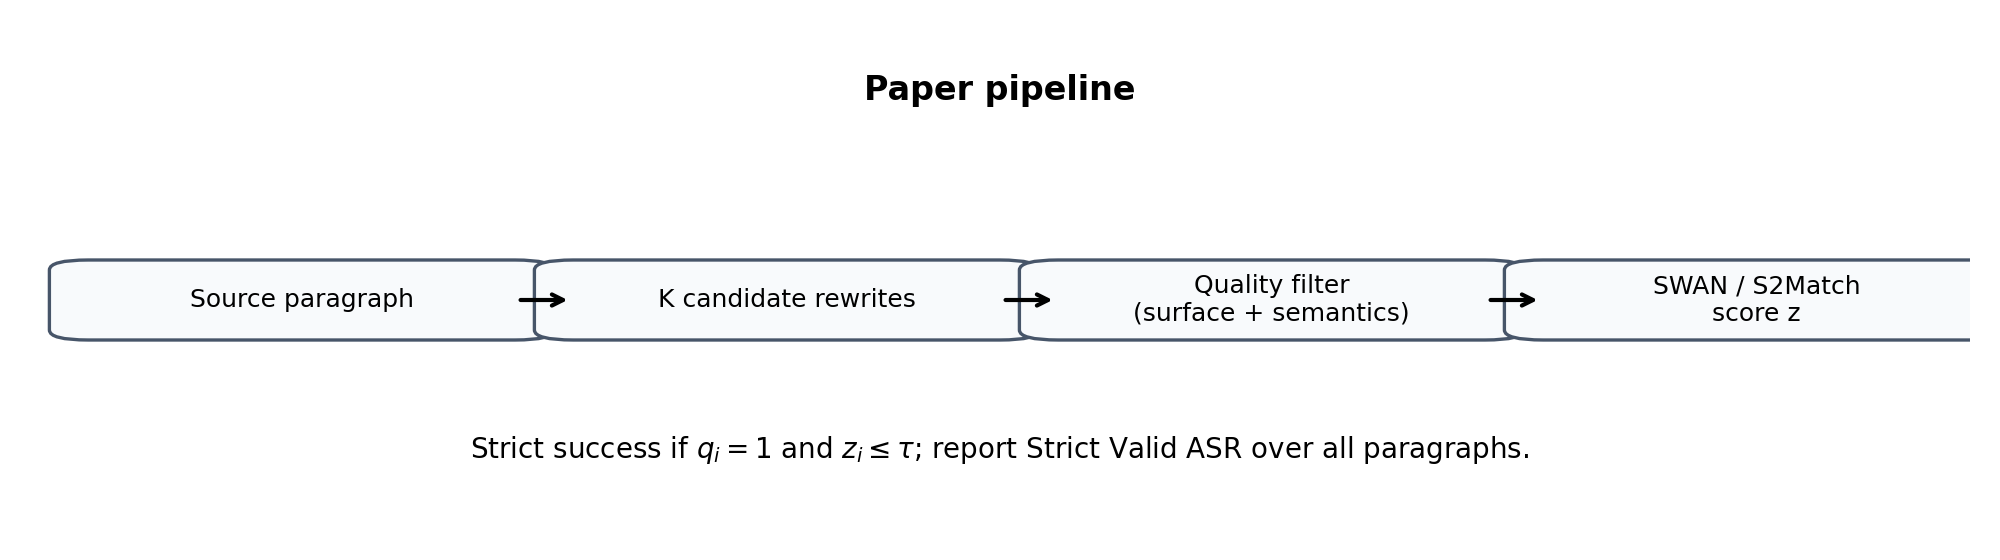
\includegraphics[width=0.92\linewidth]{figures/fig1_pipeline.png}
\caption{End-to-end experimental pipeline.}
\label{fig:pipeline}
\end{figure}
